\section{Comparaison de l'expressivité d'Astral}\label{sec:valid:expressivite:comparaison}
L'algèbre Astral a été conçue pour permettre d'exprimer des requêtes continues sans ambiguïté, mais aussi pour introduire de nouveaux opérateurs afin d'étendre la puissance d'expression des requêtes continues. Dans cette section, nous analysons en détail son expressivité. En premier lieu, nous détaillons qu'Astral couvre naturellement un large ensemble des approches actuelles. Ensuite, nous analysons les opérateurs que nous avons particulièrement remodelés : les séquences de fenêtres et la manipulation temporelle.

\subsection{Expressivité générale}
Astral est inspiré de l'algèbre \textit{ACO} de \textit{STREAM}. Nous avons repris la majeure partie des idées, notamment celle d'avoir des flux et des relations, et avons appliqué des définitions plus strictes et plus précises (c.f. section~\ref{sec:valid:expressivite:modele}). Ainsi, une requête exprimée dans \textit{ACO} peut être exprimée sans difficulté en Astral.

Dans~\cite{Arasu:stream}, il est démontré que l'expressivité de \textit{STREAM} couvre les approches de précédentes comme \textit{Chronicles}, \textit{Tribeca}, \textit{NiagaraCQ} ou \textit{Aurora}. Nous pouvons considérer qu'Astral couvre aussi ces travaux.

Notre formalisation à base de \textit{batchs} permet de supporter les sémantiques exposées par~\cite{Jain:spread}. Nous avons de même présenté notre interprétation des opérateurs \textit{SPREAD} en remplaçant les choix non déterministes par des choix sur l'ordre positionnel.

Ainsi, Astral couvre l'expressivité de plusieurs approches actuelles. Afin d'étudier ceci en détail, nous nous concentrons maintenant sur l'opérateur le plus étudié de la littérature : les séquences de fenêtres.

\subsection{Fenêtres}
Dans cette section, nous analysons l'expressivité des séquences de fenêtres. Afin de voir les capacités de notre formalisation, nous revisitons les expressions de fenêtres présentes dans l'état de l'art. Nous commençons par la plus largement utilisée : la fenêtre glissante \textit{RANGE}/\textit{SLIDE}.
\subsubsection{RANGE $x$ SLIDE $y$}
Il existe deux descriptions possibles en Astral pour cette fenêtre glissante. Ces définitions permettent d'exprimer la \textit{phase} d'initialisation. La première définition correspond à celle présente dans plusieurs travaux comme~\cite{Jain:spread} :

\DSF{r = y}{\beta(j) = yj+t_0}{\alpha(j) = \max(yj-x,0)+t_0}

Les premiers états des bornes ont une largeur de fenêtre plus petite que $x$. Dès que $j \geq \frac xy$, alors la largeur temporelle devient égale à $x$. Nous pouvons noter que la fonction $\alpha(j) = yj-x+t_0$ n'est pas valide dans notre contexte. La seconde condition des DSF (def~\ref{def:dsf}) nécessite $\alpha \geq t_0$, ce qui n'est pas vrai pour $i=0$. L'insertion de la fonction $\max$ rend la description valide et décrit la sémantique des premières phases, ce qui n'est pas explicite dans la description textuelle et dans les descriptions de la littérature.

La description suivante est aussi valide, mais ne possède pas de phase initiale. La relation temporelle est vide jusque $\beta(0)$ afin d'assurer que la fenêtre couvre toujours une largeur temporelle de $x$.

\DSF{r = y}
	{\beta(j) = yj+x+t_0}
	{\alpha(j) = yj+t_0}

Afin d'illustrer les différences entre les deux sémantiques possibles, la figure~\ref{fig:valid:expressivite:slidemax} représente les différences d'évaluations pour une fenêtre glissante avec $y=2$ et $x=4$. Dans le premier cas ($\max$), il y a deux autres évaluations à $i=0$ et $i=1$. Après cette partie, les deux modèles sont identiques.

\begin{figure}[ht]
\centering
\def\lgrad#1{\draw [thick] (#1,0) -- (#1,-0.2); \node [below] at (#1,-0.2){#1};}
\def\seg#1#2#3#4#5{\draw [thick] (#1#40.1,#3+0.25) -- (#1,#3+0.25) -- (#1,#3-0.25) -- (#1#40.1,#3-0.25); \draw [thick] (#1,#3) -- (#2,#3); \draw [thick] (#2#50.1,#3+0.25) -- (#2,#3+0.25) -- (#2,#3-0.25) -- (#2#50.1,#3-0.25);}
\def\seglbl#1#2#3#4#5#6{\seg{#1}{#2}{#3}{#4}{#5}\node [above] at (0.5*#1+0.5*#2,#3){#6};}
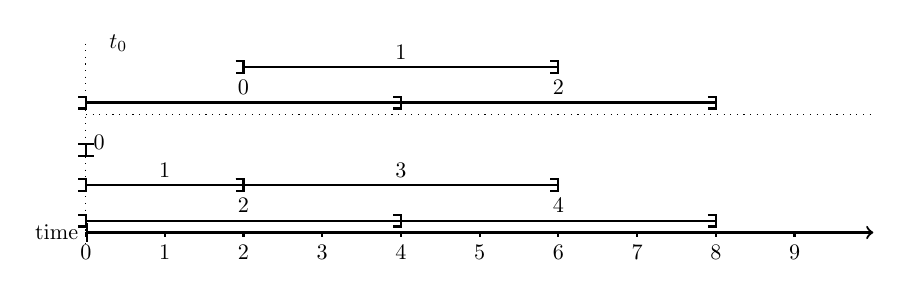
\begin{tikzpicture}[xscale=1, yscale=0.3, every node/.style={scale=0.8}]
\node [left] at (0,0) {time};
\draw [thick,|->] (0,0) -- (10,0);

\seg{0}{0}{3.5}-+\node [right] at (0,3.8){0};
\seglbl{0}{2}{2}--{1};
\seglbl{0}{4}{0.5}--{2};
\seglbl{2}{6}{2}--{3};
\seglbl{4}{8}{0.5}--{4};
\draw [dotted] (0,8) -- (0,-0.5); \node [right] at (0.2,8) {$t_0$};

\seglbl{4}{8}{5.5}--{2};
\seglbl{2}{6}{7}--{1};
\seglbl{0}{4}{5.5}--{0};
\draw [dotted] (0,5) -- (10,5);
\lgrad{0} \lgrad{1} \lgrad{2} \lgrad{3} \lgrad{4} \lgrad{5} \lgrad{6} \lgrad{7} \lgrad{8} \lgrad{9} 
\end{tikzpicture}
\caption{Différence entre les sémantiques lors de la phase d'initialisation de la fenêtre RANGE 4 SLIDE 2}\label{fig:valid:expressivite:slidemax}
\end{figure}

Nous pouvons remarquer que nous avons aussi introduit la notion d'inclusion de bornes. Ce qui permet de clarifier si la borne inférieure est incluse dans le contenu de la fenêtre. Dans le cadre des fenêtres glissantes, ce n'est pas le cas~\footnote{Il est intéressant de noter un erratum dans la spécification de cet opérateur dans~\cite{Jain:spread} où la définition précise que la borne inférieure est incluse alors que les exemples et les expérimentations pratiques indiquent le contraire.}.

\subsubsection{RANGE $x$}
Dans ses définitions usuelles, la séquence de fenêtre RANGE $x$ est similaire à RANGE $x$ SLIDE 1 ce qui est dépendant du système d'implémentation. Dans Astral, le temps n'est pas discret et une telle définition n'a pas de sens. Une définition similaire est possible en supposant que le \textit{chronon} du système d'implémentation est $\varepsilon$, alors : RANGE $x$ = RANGE $x$ SLIDE $\varepsilon$.

Une approche plus propre serait d'utiliser une DSF générique en basant ses instants d'évaluations (fournis par $\gamma$, pour rappel) sur les arrivées et départs de n-uplets dans la fenêtre. Toutefois, une connaissance de $\alpha^{-1}$ et $\beta^{-1}$ est nécessaire et rend son expression plus complexe. Il est intéressant de voir que ce comportement est similaire aux implémentations existantes. En effet, un opérateur n'est pas efficace s'il vérifie à chaque \textit{timestamp} système si un n-uplet doit sortir de la fenêtre. Il est plus efficace de planifier (via le \textit{scheduler}) ses instants d'évaluations. Ainsi, à la réception d'un n-uplet à $\tau=42$, l'opérateur planifie une exécution à $42+x$ pour faire sortir le n-uplet de la fenêtre.

\subsubsection{Descriptions à bornes linéaires}
Dans SStreamWare~\cite{Gurgen:sstreamware}, les fenêtres sont définies par un 5-uplet (start, end, rate, start\_adv, end \_adv) :
\begin{itemize}
	\item start (resp. end) décrit la borne inférieure (resp. supérieure) de la première fenêtre produite par la séquence
	\item rate est la fréquence d'évaluation
	\item start\_adv (resp. end\_adv) décrit la quantité de glissement de la borne inférieure (resp. supérieure) à chaque évaluation.
\end{itemize}

Dans Astral, ce comportement est facilement représentable sous forme de DSF :
\DSF{r = \textrm{rate}}
	{\beta(j) = \textrm{end\_adv}*j+\textrm{end}}
	{\alpha(j) = \textrm{start\_adv}*j+\textrm{start}}

\subsubsection{Descriptions procédurales}
Dans les premières versions de TelegraphCQ~\cite{Chandrasekaran:telegraphcq}, les descriptions de fenêtres étaient faites par une boucle \textit{for} procédurale sur un \textit{timestamp} :
\begin{lstlisting}[language=C]
for(t = init ; continue(t) ; t = evolution(t))
	WindowIs(S, begin(t), end(t))
\end{lstlisting}

Ceci peut être formalisé grâce à une DSF générique. Considérons la suite : $$u_n= \begin{cases} \mathrm{init} & \textrm{ si } n=0 \\ \mathrm{evolution}(u_{n-1}) & \textrm{ si } \mathrm{continue}(u_{n-1}) \\ u_{n-1} & \textrm{ sinon} \end{cases}$$

\DSF{\gamma(t,i) = \displaystyle\sum_{i=0}^{+\infty} u_i \indic_{[u_i, u_{i+1}[}(t)}
	{\beta = \textrm{end}}
	{\alpha = \textrm{begin}}

La fonction $\gamma$ est définie par une liste de points. Cette définition est courante créer des fonctions en escaliers. Il est notable que pour des fenêtres avec un taux d'évaluation constant et une position initiale usuelle, une DSF simplifiée est suffisante. 
\subsubsection{Description multidomaines}
Dans certains systèmes d'observations~\cite{Jurdak:sumac}, il est courant de récupérer les données par vagues. Ainsi, dans les interfaces de ces systèmes il est courant de trouver des séquences de fenêtres telles que \enquote{les $n$ derniers n-uples toutes les $m$ secondes}. Ces descriptions ont pour particularité d'être temporelles et positionnelles. Pour formaliser une telle séquence, il n'est pas nécessaire d'utiliser une DSF générique, car l'évaluation reste périodique. Voici la description de cette séquence de fenêtre :

\DSF{r=m}
	{\beta(j) = \rtau(mj+t_0)}
	{\alpha(j)= \max(\rtau_S(mj+t_0)-n,0)}

Le taux est temporel et les bornes sont positionnelles. Le pont entre les domaines est assuré grâce aux fonctions $\tau_S$ et $\rtau_S$. Dans ce cas, l'expression $\rtau_S(mi+t_0)$ donne la position à un \textit{timestamp} donné. La remarque concernant le $\max$ que nous avions faite plus tôt reste valable ici.

\subsubsection{Introduction d'un délai}
Dans les travaux de Patroumpas et Sellis~\cite{Patroumpas:window}, l'introduction d'un délai de traitement a été formalisée. En effet, si un n-uplet possède un \textit{timestamp} légèrement déphasé par rapport à son temps réel, alors la fenêtre peut tout de même l'inclure.

La formalisation dans notre cas revient à légèrement changer notre fonction $\gamma$ par $\gamma'$ qui décale l'évaluation de $\delta$. Par exemple, nous obtenons pour une description temporelle : $$\gamma'(t,i) = \gamma(t-\delta,i) = \left\lfloor\frac{t-\beta(0)-\delta}{r}\right\rfloor$$

\subsubsection{Modèle d'exécution de SECRET}
Enfin, SECRET~\cite{Botan:secret} est un modèle permettant de généraliser les sémantiques d'exécutions des fenêtres. L'approche est de découper l'exécution d'une fenêtre en quatre concepts que nous pouvons retrouver dans Astral.
\begin{itemize}
	\item Les \textit{Ticks} décident du moment où le système doit réagir au flux (sémantique basée n-uplet, basé temps ou \textit{batch}).
	\item Le \textit{Content} défini le contenu global de la fenêtre par son \textit{Scope}, c'est-à-dire sa description.
	\item Enfin, un \textit{Report} envoie le résultat final.
\end{itemize}

Bien que les approches soient différentes : nous retrouvons des notions similaires. Le \textit{Scope} est similaire à $\alpha$, $\beta$. Le \textit{Content} est assimilable à une fenêtre en particulier. Les \textit{Ticks} et les \textit{Reports} sont faits grâce à la fonction $\gamma$ et le contrôle du mode d'exécution par les opérateurs \textit{SPREAD}. L'avantage de l'approche de SECRET est de pouvoir qualifier rapidement le comportement de l'exécution d'un SGFD en particulier, alors qu'Astral décrit la sémantique exacte du résultat pour l'utilisateur.

Nous avons détaillé le positionnement de l'opérateur de séquence de fenêtre par rapport à la littérature. Nous constatons que l'opérateur permet de couvrir l'ensemble des sémantiques. Nous avons clarifié plusieurs descriptions non triviales telles que les fenêtres RANGE strictes, les fenêtres multidomaines et l'introduction du délai. Nous présentons maintenant l'analyse de l'opérateur de manipulation temporelle.

\subsubsection{ROWS $x$ SLIDE $y$}
Nous avons présenté dans le tableau~\ref{tab:windows} que la séquence de fenêtre positionnelle décrivant les $x$ derniers n-uplets tous les $y$ n-uplets est une description linéaire. Cette description reflète la sémantique de \textit{ROWS} de dans la plupart des cas. Toutefois, lors que le nombre de n-uplets par \textit{batch} est plus grand que $y$ et non proportionnel à $y$, alors les descriptions diffèrent.

Soit un flux $S$ ayant les batchs suivants $@b_1=\{s_1, s_2, s_3\}$, $@b_2=\{s_4\}$, $@b_3=\{s_5\}$. Nous souhaitons appliquer l'opérateur $]P\ 2\ 2]$. Nous obtenons pour $b_1$ la sélection des deux n-uplets les plus récents du batch contenant les n-uplets 1 et 2. Pour $b_2$, nous sélectionnons les n-uplets 3 et 4. Selon~\cite{Jain:spread}, la sémantique de $[$ROWS $x$ SLIDE $y]$ est pour $b_1$ : deux n-uplets du dernier batch, et pour $b_3$ les deux n-uplets suivants. Un décalage a été introduit pour permettre de ne pas utiliser deux fois le même \textit{batch} ce qui rend la description non linéaire. Le tableau suivant compare les deux descriptions :

\begin{center}
\begin{tabular}{|c|c|c|} \bottomrule
batch & $]P\ 2\ 2]$ & $[$ROWS $x$ SLIDE $y]$\\ \hline
$b_1$ & $\{s_2,s_3\}$ & $\{s_2,s_3\}$ ou $\{s_1,s_3\}$ ou $\{s_1,s_2\}$ \\\hline
$b_2$ & $\{s_3,s_4\}$ & comme $b_1$ \\\hline
$b_3$ & comme $b_2$ & $\{s_4,s_5\}$ \\ \toprule
\end{tabular}
\end{center}

Il est toutefois possible de retrouver cette description grâce à l'introduction d'un décalage suivant le \textit{modulo} des cardinalités des \textit{batchs} rencontrés à $n*y$ : $$\delta_j = \left(\sum_{n=0}^j \rtau_S\circ \tau_S(yn)\right) \bmod y$$
Il suffit d'ajouter ce $\delta_j$ aux expressions d'$\alpha$ et $\beta$ et nous retrouvons le même comportement que la description $[$ROWS $x$ SLIDE $y]$. Enfin, la sémantique de ROWS $x$ est équivalente à $y=1$.
 
\subsection{Manipulation temporelle}
L'opérateur de manipulation temporelle (définition~\ref{def:manipulation}) permet de donner à une relation temporelle un état qu'elle a eu précédemment. Ceci permet de transformer le moment d'évaluation de la relation temporelle. Dans l'état de l'art, à notre connaissance, il n'existe pas d'opérateur capable d'exprimer explicitement cette opération.

Cet opérateur nous a permis notamment d'introduire la jointure semi-sensible $\ssjoin$ (définition~\ref{def:ssjoin}). Cette jointure permet de refléter un comportement qui se retrouve dans plusieurs SGFD : ne réagir que sur les mises à jour d'une seule branche d'une opération de jointure.

Une autre application intéressante de l'opérateur de manipulation temporelle est le calcul de changement d'une relation temporelle. Comme nous l'avons vu, l'opérateur $\IS$ est capable de créer un flux composé des nouveaux n-uplets d'une relation. Dans le cadre l'observation de système, nous pouvons réaliser l'opération suivante : \enquote{A partir d'une relation temporelle $R$($id$,$v$), fournir le flux des changements ($id$,$v$,$v_{old}$) où $v_{old}$ est l'ancienne valeur $v$ pour l'identifiant $id$}. Cette requête s'écrit ainsi :
$$\IS(R \Join_{v\neq v_{old}} (D^{(t,i)^-}_{t>t_0}\rho_{v_{old}/v} R))$$
L'opérateur $D^{(t,i)^-}_{t>t_0}$ \enquote{retarde} la relation temporelle d'un \textit{batch}. Il devient possible d'interroger à un instant donné, une relation temporelle et son état précédent.

Nous avons présenté l'ensemble des aspects novateurs des définitions d'Astral. Nous détaillons maintenant les propriétés de cette algèbre avec un ensemble de propositions et de théorèmes.
